\section{ODV-Bench}
\label{sec:Benchmark}


Muchos benchmarks existentes para escenarios de streaming derivan de datasets de evaluación de video offline \cite{lin2024streamingbench,huang2024videochatonline,li2025ovobench,xiong2025streamchat}, y pueden no reflejar adecuadamente aplicaciones reales de streaming video understanding. 
Aunque algunos de ellos ya incorporan videos Ego4D de actividades cotidianas \cite{li2025ovobench,xiong2025streamchat}, estas muestras de evaluación evalúan principalmente la capacidad de los MLLMs para percibir escenas estáticas y narrar interacciones humano-entorno de manera secuencial. 
En contraste, la conducción autónoma presenta entornos dinámicos de alta exigencia con escenas que cambian rápidamente, interacciones complejas entre múltiples agentes (vehículos, peatones y señales de tránsito) y tareas de predicción demandantes (como evaluación de riesgo y planificación de movimiento). Estos escenarios requieren que los modelos equilibren memoria de largo plazo de eventos con percepción fina de corto plazo para evitar accidentes y tomar decisiones oportunas. Para abordar esta brecha, introducimos ODV-Bench, un benchmark diseñado específicamente para online video understanding en escenarios de conducción autónoma.


\subsection{Formulación de tareas}
Como se muestra en la Figura \ref{fig:benchmark} (a), primero exploramos los elementos clave del tránsito en escenarios de conducción autónoma y los resumimos en tres categorías de escenarios de tarea:\textbf{ (1) tareas orientadas a objetivos estáticos}, que involucran el reconocimiento y la recuperación de elementos de tránsito estacionarios como señales, semáforos e indicadores viales; \textbf{ (2) tareas orientadas a objetivos dinámicos}, que se enfocan en la predicción de comportamiento y trayectoria de participantes dinámicos de la vía como vehículos y peatones; y \textbf{ (3) tareas orientadas a eventos para interacción multiagente}, que capturan interacciones complejas, escenarios de riesgo y accidentes que involucran múltiples agentes. Luego, guiados por señales temporales y por las necesidades prácticas de la conducción, definimos además tipos de tareas finas basadas en estas categorías para evaluar de forma integral la comprensión del modelo en escenarios realistas de video de conducción online. Para más detalles sobre la formulación de tareas, véase el Apéndice \ref{app:sec:Details_of_ODVBench:Task}.


\begin{figure*}[t]
    % \vspace{-5pt}
    \centering
    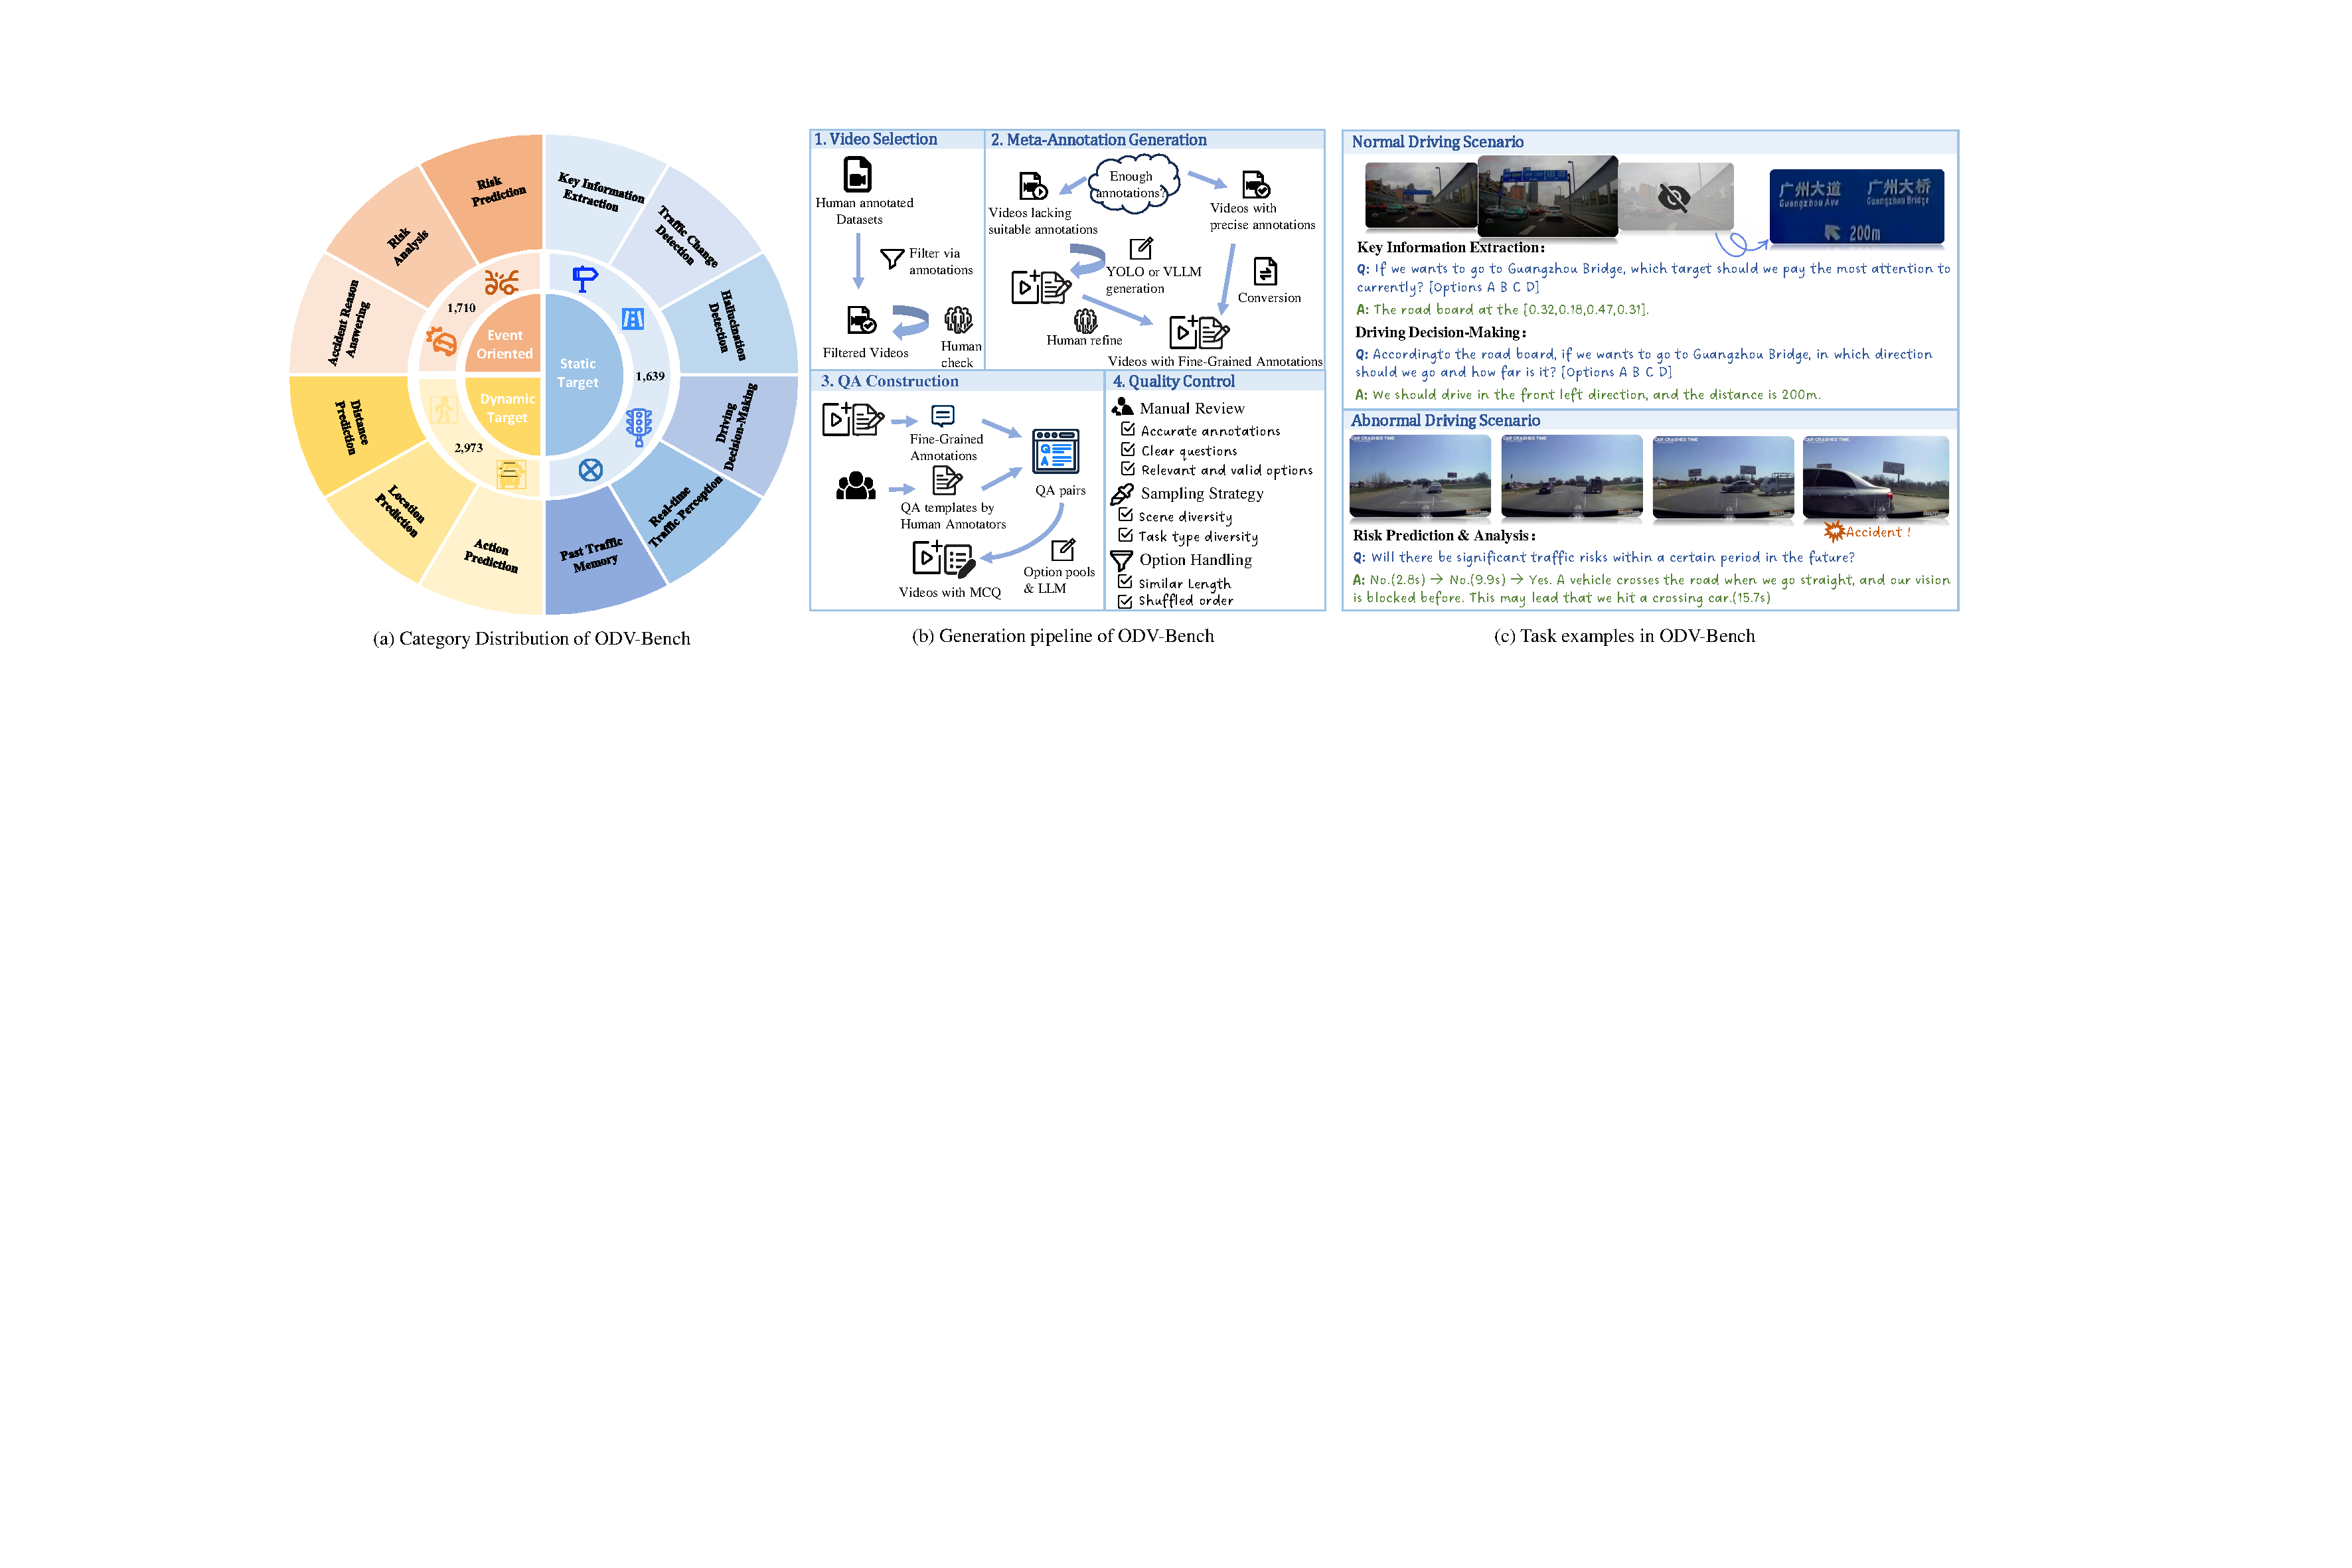
\includegraphics[width=\textwidth]{figs/benchmark_img.pdf} 
    \caption{(a) La distribución de tipos de tarea y la cantidad de pares QA. (b) El pipeline detallado para construir ODV-Bench. (c) Ejemplos típicos de tareas en ODV-Bench.
    }
    \label{fig:benchmark}
    % \vspace{-5pt}
\end{figure*}


\subsection{Construcción del benchmark}
El proceso de construcción de ODV-Bench se ilustra en la Figura \ref{fig:benchmark} (b). Adoptamos un enfoque de cuatro etapas para garantizar la calidad de cada pregunta generada, y luego presentamos algunos ejemplos típicos de tareas en distintos escenarios de conducción en la Figura \ref{fig:benchmark} (c).

\textbf{Recolección de datos.} \textbf{(1) Selección de videos.} Para alinearnos con escenarios de conducción del mundo real, primero curamos 6 datasets \cite{khan2024road,fang2024abductive,zurn2024wayvescenes101,yu2020bdd100k,zhang2023videotext,che2019d} provenientes de distintos escenarios de tarea dentro del dominio de la conducción autónoma, desde conducción normal hasta eventos inesperados. Luego diseñamos una tubería semiautomática que se apoya principalmente en filtrado de anotaciones y detección basada en YOLO \cite{khanam2024yolov11}, complementada con inspección manual, para seleccionar videos relevantes para la tarea del dataset recolectado. \textbf{(2) Generación de meta-anotaciones.} Para obtener meta-anotaciones con información espaciotemporal y semántica detallada, desarrollamos métodos a medida basados en anotaciones existentes de los datasets. Para datasets bien anotados, convertimos eficazmente las etiquetas existentes en meta-anotaciones específicas de la tarea. Para los demás, diseñamos una tubería semiautomática que comienza con anotaciones gruesas generadas por VLLM y YOLO \cite{khanam2024yolov11}, seguidas por verificación humana estructurada para garantizar calidad.

\textbf{Construcción de QA.} \textbf{(1) Generación de MCQ.} Para habilitar generación automática eficiente de QA, primero diseñamos plantillas precisas y diversas adaptadas a cada tarea definida. Estas plantillas se completan luego con anotaciones finas y precisas para generar pares QA de alta calidad. Después desarrollamos una tubería de generación de múltiple opción basada en un conjunto de opciones, introduciendo distractores plausibles pero engañosos junto con la respuesta correcta para asegurar el realismo y la efectividad de las opciones. \textbf{(2) Control de calidad.} Para garantizar la calidad del benchmark, primero realizamos múltiples rondas de revisión manual para verificar la claridad y exactitud de los pares QA y la plausibilidad de las opciones distractoras. Además, para mejorar la diversidad de escenas y el equilibrio entre tipos de tareas, aplicamos una estrategia de muestreo que asigna preguntas proporcionalmente a la longitud del video, maximizando la cobertura entre escenarios.
